% Created by tikzDevice version 0.12.3.1 on 2021-07-03 12:16:23
% !TEX encoding = UTF-8 Unicode
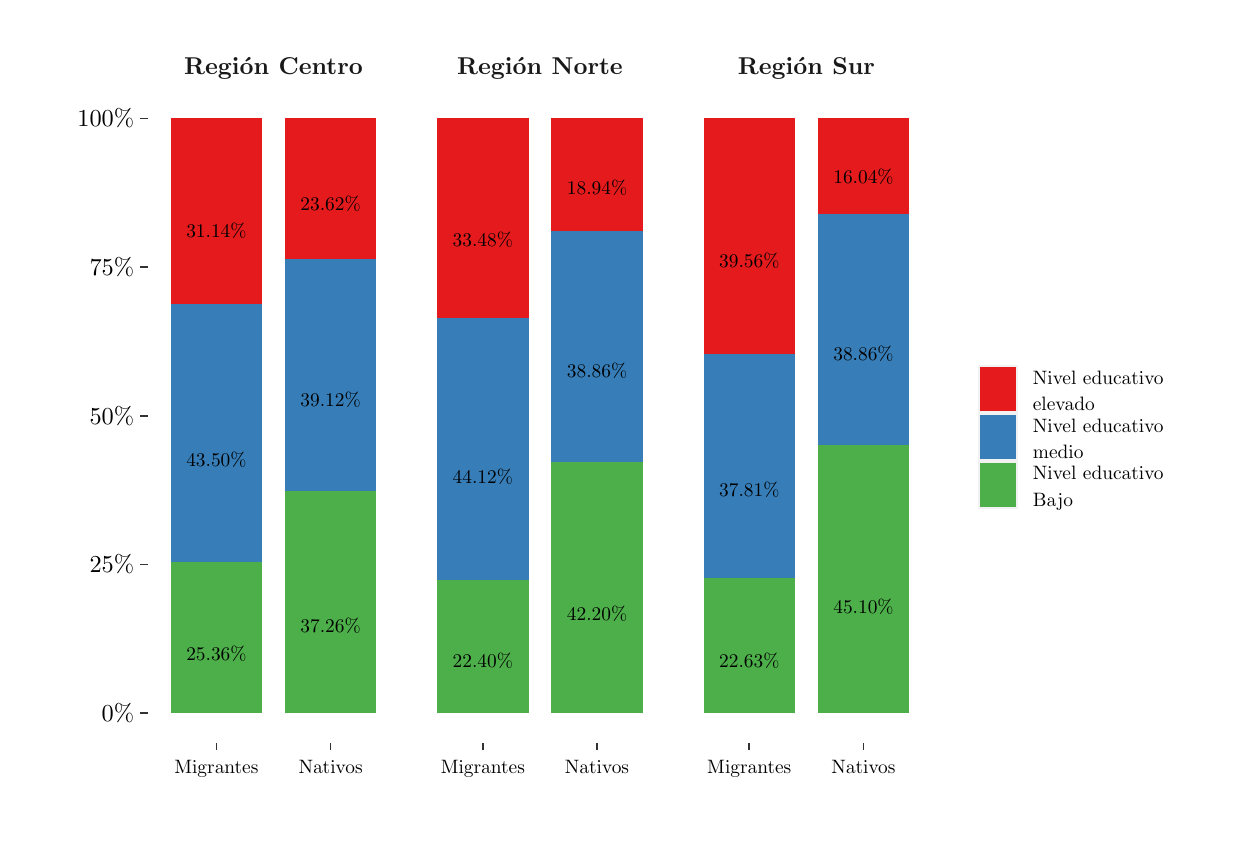
\begin{tikzpicture}[x=1pt,y=1pt]
\definecolor{fillColor}{RGB}{255,255,255}
\path[use as bounding box,fill=fillColor,fill opacity=0.00] (0,0) rectangle (433.62,289.08);
\begin{scope}
\path[clip] (  0.00,  0.00) rectangle (433.62,289.08);
\definecolor{drawColor}{RGB}{255,255,255}
\definecolor{fillColor}{RGB}{255,255,255}

\path[draw=drawColor,line width= 0.6pt,line join=round,line cap=round,fill=fillColor] (  0.00,  0.00) rectangle (433.62,289.08);
\end{scope}
\begin{scope}
\path[clip] ( 43.44, 30.69) rectangle (134.22,267.01);
\definecolor{drawColor}{RGB}{255,255,255}

\path[draw=drawColor,line width= 0.3pt,line join=round] ( 43.44, 68.28) --
	(134.22, 68.28);

\path[draw=drawColor,line width= 0.3pt,line join=round] ( 43.44,121.99) --
	(134.22,121.99);

\path[draw=drawColor,line width= 0.3pt,line join=round] ( 43.44,175.70) --
	(134.22,175.70);

\path[draw=drawColor,line width= 0.3pt,line join=round] ( 43.44,229.41) --
	(134.22,229.41);

\path[draw=drawColor,line width= 0.6pt,line join=round] ( 43.44, 41.43) --
	(134.22, 41.43);

\path[draw=drawColor,line width= 0.6pt,line join=round] ( 43.44, 95.14) --
	(134.22, 95.14);

\path[draw=drawColor,line width= 0.6pt,line join=round] ( 43.44,148.85) --
	(134.22,148.85);

\path[draw=drawColor,line width= 0.6pt,line join=round] ( 43.44,202.56) --
	(134.22,202.56);

\path[draw=drawColor,line width= 0.6pt,line join=round] ( 43.44,256.27) --
	(134.22,256.27);

\path[draw=drawColor,line width= 0.6pt,line join=round] ( 68.20, 30.69) --
	( 68.20,267.01);

\path[draw=drawColor,line width= 0.6pt,line join=round] (109.46, 30.69) --
	(109.46,267.01);
\definecolor{fillColor}{RGB}{228,26,28}

\path[fill=fillColor] ( 51.70,189.37) rectangle ( 84.71,256.27);
\definecolor{fillColor}{RGB}{55,126,184}

\path[fill=fillColor] ( 51.70, 95.92) rectangle ( 84.71,189.37);
\definecolor{fillColor}{RGB}{77,175,74}

\path[fill=fillColor] ( 51.70, 41.43) rectangle ( 84.71, 95.92);
\definecolor{fillColor}{RGB}{228,26,28}

\path[fill=fillColor] ( 92.96,205.52) rectangle (125.97,256.27);
\definecolor{fillColor}{RGB}{55,126,184}

\path[fill=fillColor] ( 92.96,121.48) rectangle (125.97,205.52);
\definecolor{fillColor}{RGB}{77,175,74}

\path[fill=fillColor] ( 92.96, 41.43) rectangle (125.97,121.48);
\definecolor{drawColor}{RGB}{0,0,0}

\node[text=drawColor,anchor=base,inner sep=0pt, outer sep=0pt, scale=  0.70] at ( 68.20,213.19) {31.14{\%}};

\node[text=drawColor,anchor=base,inner sep=0pt, outer sep=0pt, scale=  0.70] at ( 68.20,130.36) {43.50{\%}};

\node[text=drawColor,anchor=base,inner sep=0pt, outer sep=0pt, scale=  0.70] at ( 68.20, 60.28) {25.36{\%}};

\node[text=drawColor,anchor=base,inner sep=0pt, outer sep=0pt, scale=  0.70] at (109.46,222.88) {23.62{\%}};

\node[text=drawColor,anchor=base,inner sep=0pt, outer sep=0pt, scale=  0.70] at (109.46,152.15) {39.12{\%}};

\node[text=drawColor,anchor=base,inner sep=0pt, outer sep=0pt, scale=  0.70] at (109.46, 70.51) {37.26{\%}};
\end{scope}
\begin{scope}
\path[clip] (139.72, 30.69) rectangle (230.50,267.01);
\definecolor{drawColor}{RGB}{255,255,255}

\path[draw=drawColor,line width= 0.3pt,line join=round] (139.72, 68.28) --
	(230.50, 68.28);

\path[draw=drawColor,line width= 0.3pt,line join=round] (139.72,121.99) --
	(230.50,121.99);

\path[draw=drawColor,line width= 0.3pt,line join=round] (139.72,175.70) --
	(230.50,175.70);

\path[draw=drawColor,line width= 0.3pt,line join=round] (139.72,229.41) --
	(230.50,229.41);

\path[draw=drawColor,line width= 0.6pt,line join=round] (139.72, 41.43) --
	(230.50, 41.43);

\path[draw=drawColor,line width= 0.6pt,line join=round] (139.72, 95.14) --
	(230.50, 95.14);

\path[draw=drawColor,line width= 0.6pt,line join=round] (139.72,148.85) --
	(230.50,148.85);

\path[draw=drawColor,line width= 0.6pt,line join=round] (139.72,202.56) --
	(230.50,202.56);

\path[draw=drawColor,line width= 0.6pt,line join=round] (139.72,256.27) --
	(230.50,256.27);

\path[draw=drawColor,line width= 0.6pt,line join=round] (164.48, 30.69) --
	(164.48,267.01);

\path[draw=drawColor,line width= 0.6pt,line join=round] (205.74, 30.69) --
	(205.74,267.01);
\definecolor{fillColor}{RGB}{228,26,28}

\path[fill=fillColor] (147.97,184.34) rectangle (180.99,256.27);
\definecolor{fillColor}{RGB}{55,126,184}

\path[fill=fillColor] (147.97, 89.55) rectangle (180.99,184.34);
\definecolor{fillColor}{RGB}{77,175,74}

\path[fill=fillColor] (147.97, 41.43) rectangle (180.99, 89.55);
\definecolor{fillColor}{RGB}{228,26,28}

\path[fill=fillColor] (189.24,215.57) rectangle (222.25,256.27);
\definecolor{fillColor}{RGB}{55,126,184}

\path[fill=fillColor] (189.24,132.09) rectangle (222.25,215.57);
\definecolor{fillColor}{RGB}{77,175,74}

\path[fill=fillColor] (189.24, 41.43) rectangle (222.25,132.09);
\definecolor{drawColor}{RGB}{0,0,0}

\node[text=drawColor,anchor=base,inner sep=0pt, outer sep=0pt, scale=  0.70] at (164.48,210.17) {33.48{\%}};

\node[text=drawColor,anchor=base,inner sep=0pt, outer sep=0pt, scale=  0.70] at (164.48,124.53) {44.12{\%}};

\node[text=drawColor,anchor=base,inner sep=0pt, outer sep=0pt, scale=  0.70] at (164.48, 57.74) {22.40{\%}};

\node[text=drawColor,anchor=base,inner sep=0pt, outer sep=0pt, scale=  0.70] at (205.74,228.91) {18.94{\%}};

\node[text=drawColor,anchor=base,inner sep=0pt, outer sep=0pt, scale=  0.70] at (205.74,162.54) {38.86{\%}};

\node[text=drawColor,anchor=base,inner sep=0pt, outer sep=0pt, scale=  0.70] at (205.74, 74.75) {42.20{\%}};
\end{scope}
\begin{scope}
\path[clip] (236.00, 30.69) rectangle (326.78,267.01);
\definecolor{drawColor}{RGB}{255,255,255}

\path[draw=drawColor,line width= 0.3pt,line join=round] (236.00, 68.28) --
	(326.78, 68.28);

\path[draw=drawColor,line width= 0.3pt,line join=round] (236.00,121.99) --
	(326.78,121.99);

\path[draw=drawColor,line width= 0.3pt,line join=round] (236.00,175.70) --
	(326.78,175.70);

\path[draw=drawColor,line width= 0.3pt,line join=round] (236.00,229.41) --
	(326.78,229.41);

\path[draw=drawColor,line width= 0.6pt,line join=round] (236.00, 41.43) --
	(326.78, 41.43);

\path[draw=drawColor,line width= 0.6pt,line join=round] (236.00, 95.14) --
	(326.78, 95.14);

\path[draw=drawColor,line width= 0.6pt,line join=round] (236.00,148.85) --
	(326.78,148.85);

\path[draw=drawColor,line width= 0.6pt,line join=round] (236.00,202.56) --
	(326.78,202.56);

\path[draw=drawColor,line width= 0.6pt,line join=round] (236.00,256.27) --
	(326.78,256.27);

\path[draw=drawColor,line width= 0.6pt,line join=round] (260.76, 30.69) --
	(260.76,267.01);

\path[draw=drawColor,line width= 0.6pt,line join=round] (302.02, 30.69) --
	(302.02,267.01);
\definecolor{fillColor}{RGB}{228,26,28}

\path[fill=fillColor] (244.25,171.28) rectangle (277.26,256.27);
\definecolor{fillColor}{RGB}{55,126,184}

\path[fill=fillColor] (244.25, 90.05) rectangle (277.26,171.28);
\definecolor{fillColor}{RGB}{77,175,74}

\path[fill=fillColor] (244.25, 41.43) rectangle (277.26, 90.05);
\definecolor{fillColor}{RGB}{228,26,28}

\path[fill=fillColor] (285.52,221.81) rectangle (318.53,256.27);
\definecolor{fillColor}{RGB}{55,126,184}

\path[fill=fillColor] (285.52,138.33) rectangle (318.53,221.81);
\definecolor{fillColor}{RGB}{77,175,74}

\path[fill=fillColor] (285.52, 41.43) rectangle (318.53,138.33);
\definecolor{drawColor}{RGB}{0,0,0}

\node[text=drawColor,anchor=base,inner sep=0pt, outer sep=0pt, scale=  0.70] at (260.76,202.33) {39.56{\%}};

\node[text=drawColor,anchor=base,inner sep=0pt, outer sep=0pt, scale=  0.70] at (260.76,119.60) {37.81{\%}};

\node[text=drawColor,anchor=base,inner sep=0pt, outer sep=0pt, scale=  0.70] at (260.76, 57.94) {22.63{\%}};

\node[text=drawColor,anchor=base,inner sep=0pt, outer sep=0pt, scale=  0.70] at (302.02,232.65) {16.04{\%}};

\node[text=drawColor,anchor=base,inner sep=0pt, outer sep=0pt, scale=  0.70] at (302.02,168.78) {38.86{\%}};

\node[text=drawColor,anchor=base,inner sep=0pt, outer sep=0pt, scale=  0.70] at (302.02, 77.25) {45.10{\%}};
\end{scope}
\begin{scope}
\path[clip] ( 43.44,267.01) rectangle (134.22,283.58);
\definecolor{drawColor}{gray}{0.10}

\node[text=drawColor,anchor=base,inner sep=0pt, outer sep=0pt, scale=  0.88] at ( 88.83,272.26) {\textbf{Región Centro}};
\end{scope}
\begin{scope}
\path[clip] (139.72,267.01) rectangle (230.50,283.58);
\definecolor{drawColor}{gray}{0.10}

\node[text=drawColor,anchor=base,inner sep=0pt, outer sep=0pt, scale=  0.88] at (185.11,272.26) {\textbf{Región Norte}};
\end{scope}
\begin{scope}
\path[clip] (236.00,267.01) rectangle (326.78,283.58);
\definecolor{drawColor}{gray}{0.10}

\node[text=drawColor,anchor=base,inner sep=0pt, outer sep=0pt, scale=  0.88] at (281.39,272.26) {\textbf{Región Sur}};
\end{scope}
\begin{scope}
\path[clip] (  0.00,  0.00) rectangle (433.62,289.08);
\definecolor{drawColor}{gray}{0.20}

\path[draw=drawColor,line width= 0.6pt,line join=round] ( 68.20, 27.94) --
	( 68.20, 30.69);

\path[draw=drawColor,line width= 0.6pt,line join=round] (109.46, 27.94) --
	(109.46, 30.69);
\end{scope}
\begin{scope}
\path[clip] (  0.00,  0.00) rectangle (433.62,289.08);
\definecolor{drawColor}{RGB}{0,0,0}

\node[text=drawColor,anchor=base,inner sep=0pt, outer sep=0pt, scale=  0.70] at ( 68.20, 19.68) {Migrantes};

\node[text=drawColor,anchor=base,inner sep=0pt, outer sep=0pt, scale=  0.70] at (109.46, 19.68) {Nativos};
\end{scope}
\begin{scope}
\path[clip] (  0.00,  0.00) rectangle (433.62,289.08);
\definecolor{drawColor}{gray}{0.20}

\path[draw=drawColor,line width= 0.6pt,line join=round] (164.48, 27.94) --
	(164.48, 30.69);

\path[draw=drawColor,line width= 0.6pt,line join=round] (205.74, 27.94) --
	(205.74, 30.69);
\end{scope}
\begin{scope}
\path[clip] (  0.00,  0.00) rectangle (433.62,289.08);
\definecolor{drawColor}{RGB}{0,0,0}

\node[text=drawColor,anchor=base,inner sep=0pt, outer sep=0pt, scale=  0.70] at (164.48, 19.68) {Migrantes};

\node[text=drawColor,anchor=base,inner sep=0pt, outer sep=0pt, scale=  0.70] at (205.74, 19.68) {Nativos};
\end{scope}
\begin{scope}
\path[clip] (  0.00,  0.00) rectangle (433.62,289.08);
\definecolor{drawColor}{gray}{0.20}

\path[draw=drawColor,line width= 0.6pt,line join=round] (260.76, 27.94) --
	(260.76, 30.69);

\path[draw=drawColor,line width= 0.6pt,line join=round] (302.02, 27.94) --
	(302.02, 30.69);
\end{scope}
\begin{scope}
\path[clip] (  0.00,  0.00) rectangle (433.62,289.08);
\definecolor{drawColor}{RGB}{0,0,0}

\node[text=drawColor,anchor=base,inner sep=0pt, outer sep=0pt, scale=  0.70] at (260.76, 19.68) {Migrantes};

\node[text=drawColor,anchor=base,inner sep=0pt, outer sep=0pt, scale=  0.70] at (302.02, 19.68) {Nativos};
\end{scope}
\begin{scope}
\path[clip] (  0.00,  0.00) rectangle (433.62,289.08);
\definecolor{drawColor}{RGB}{0,0,0}

\node[text=drawColor,anchor=base east,inner sep=0pt, outer sep=0pt, scale=  0.88] at ( 38.49, 38.40) {0{\%}};

\node[text=drawColor,anchor=base east,inner sep=0pt, outer sep=0pt, scale=  0.88] at ( 38.49, 92.11) {25{\%}};

\node[text=drawColor,anchor=base east,inner sep=0pt, outer sep=0pt, scale=  0.88] at ( 38.49,145.82) {50{\%}};

\node[text=drawColor,anchor=base east,inner sep=0pt, outer sep=0pt, scale=  0.88] at ( 38.49,199.53) {75{\%}};

\node[text=drawColor,anchor=base east,inner sep=0pt, outer sep=0pt, scale=  0.88] at ( 38.49,253.24) {100{\%}};
\end{scope}
\begin{scope}
\path[clip] (  0.00,  0.00) rectangle (433.62,289.08);
\definecolor{drawColor}{gray}{0.20}

\path[draw=drawColor,line width= 0.6pt,line join=round] ( 40.69, 41.43) --
	( 43.44, 41.43);

\path[draw=drawColor,line width= 0.6pt,line join=round] ( 40.69, 95.14) --
	( 43.44, 95.14);

\path[draw=drawColor,line width= 0.6pt,line join=round] ( 40.69,148.85) --
	( 43.44,148.85);

\path[draw=drawColor,line width= 0.6pt,line join=round] ( 40.69,202.56) --
	( 43.44,202.56);

\path[draw=drawColor,line width= 0.6pt,line join=round] ( 40.69,256.27) --
	( 43.44,256.27);
\end{scope}
\begin{scope}
\path[clip] (  0.00,  0.00) rectangle (433.62,289.08);
\definecolor{fillColor}{RGB}{255,255,255}

\path[fill=fillColor] (337.78,109.83) rectangle (428.12,187.87);
\end{scope}
\begin{scope}
\path[clip] (  0.00,  0.00) rectangle (433.62,289.08);
\definecolor{fillColor}{gray}{0.95}

\path[fill=fillColor] (343.28,149.88) rectangle (357.73,167.15);
\end{scope}
\begin{scope}
\path[clip] (  0.00,  0.00) rectangle (433.62,289.08);
\definecolor{fillColor}{RGB}{228,26,28}

\path[fill=fillColor] (343.99,150.59) rectangle (357.02,166.44);
\end{scope}
\begin{scope}
\path[clip] (  0.00,  0.00) rectangle (433.62,289.08);
\definecolor{fillColor}{gray}{0.95}

\path[fill=fillColor] (343.28,132.60) rectangle (357.73,149.88);
\end{scope}
\begin{scope}
\path[clip] (  0.00,  0.00) rectangle (433.62,289.08);
\definecolor{fillColor}{RGB}{55,126,184}

\path[fill=fillColor] (343.99,133.31) rectangle (357.02,149.17);
\end{scope}
\begin{scope}
\path[clip] (  0.00,  0.00) rectangle (433.62,289.08);
\definecolor{fillColor}{gray}{0.95}

\path[fill=fillColor] (343.28,115.33) rectangle (357.73,132.60);
\end{scope}
\begin{scope}
\path[clip] (  0.00,  0.00) rectangle (433.62,289.08);
\definecolor{fillColor}{RGB}{77,175,74}

\path[fill=fillColor] (343.99,116.04) rectangle (357.02,131.89);
\end{scope}
\begin{scope}
\path[clip] (  0.00,  0.00) rectangle (433.62,289.08);
\definecolor{drawColor}{RGB}{0,0,0}

\node[text=drawColor,anchor=base west,inner sep=0pt, outer sep=0pt, scale=  0.70] at (363.23,160.24) {Nivel educativo};

\node[text=drawColor,anchor=base west,inner sep=0pt, outer sep=0pt, scale=  0.70] at (363.23,150.73) {elevado};
\end{scope}
\begin{scope}
\path[clip] (  0.00,  0.00) rectangle (433.62,289.08);
\definecolor{drawColor}{RGB}{0,0,0}

\node[text=drawColor,anchor=base west,inner sep=0pt, outer sep=0pt, scale=  0.70] at (363.23,142.96) {Nivel educativo};

\node[text=drawColor,anchor=base west,inner sep=0pt, outer sep=0pt, scale=  0.70] at (363.23,133.46) {medio};
\end{scope}
\begin{scope}
\path[clip] (  0.00,  0.00) rectangle (433.62,289.08);
\definecolor{drawColor}{RGB}{0,0,0}

\node[text=drawColor,anchor=base west,inner sep=0pt, outer sep=0pt, scale=  0.70] at (363.23,125.69) {Nivel educativo};

\node[text=drawColor,anchor=base west,inner sep=0pt, outer sep=0pt, scale=  0.70] at (363.23,116.18) {Bajo};
\end{scope}
\end{tikzpicture}
